\documentclass[a4paper,11pt,twoside]{article}
%\documentclass[a4paper,11pt,twoside,se]{article}

\usepackage{UmUStudentReport}
\usepackage{verbatim}   % Multi-line comments using \begin{comment}
\usepackage{courier}    % Nicer fonts are used. (not necessary)
\usepackage{pslatex}    % Also nicer fonts. (not necessary)
\usepackage[pdftex]{graphicx}   % allows including pdf figures
\usepackage{listings}
%\usepackage{lmodern}   % Optional fonts. (not necessary)
%\usepackage{tabularx}
%\usepackage{microtype} % Provides some typographic improvements over default settings
%\usepackage{placeins}  % For aligning images with \FloatBarrier
%\usepackage{booktabs}  % For nice-looking tables
%\usepackage{titlesec}  % More granular control of sections.

% DOCUMENT INFO
% =============
\department{Institution för Datavetenskap}
\coursename{DV2: Algorithms and Problemsolving 7.5 p}
\coursecode{DV169VT16}
\title{OU5 Automaton}
\author{Lorenz Gerber ({\tt{dv15lgr@cs.umu.se}} {\tt{lozger03@student.umu.se}})}
\date{2016-03-21}
%\revisiondate{2016-01-18}
\instructor{Lena Kallin Westin / Erik Moström / Jonathan Westin}


% DOCUMENT SETTINGS
% =================
\bibliographystyle{plain}
%\bibliographystyle{ieee}
\pagestyle{fancy}
\raggedbottom
\setcounter{secnumdepth}{2}
\setcounter{tocdepth}{2}
%\graphicspath{{images/}}   %Path for images

\usepackage{float}
\floatstyle{ruled}
\newfloat{listing}{thp}{lop}
\floatname{listing}{Listing}



% DEFINES
% =======
%\newcommand{\mycommand}{<latex code>}

% DOCUMENT
% ========
\begin{document}
\lstset{language=C}
\maketitle
\thispagestyle{empty}
\newpage
\tableofcontents
\thispagestyle{empty}
\newpage

\clearpage
\pagenumbering{arabic}

\section{Introduction} 
The subject of this assignment was to design and construct Push Down
Automaton (PDA) as a general datatype and apply it to implement a
specific PDA that can process input according to \textit{reverse
  polish notation} (RPN).

The formal defintion of a PDA is a 6-tuple consisting of the set of
States, the input alphabet, the stack alphabet, transition functions,
a start state and a set of accepted states. PDA's can be either
deterministic or non-deterministic. The special feature of a PDA is
the stack which allows to store information and process it later. 

RPN is a way of writing aritmethic expressions. Instead of the common
`in-fix' notation where an operator is written between the two
operands, RPN uses `post-fix' notation with the operator after the
operands. This way of indicating arithmetic expressions makes
paranthesis to modify the precedence of operators obsolete. RPN has
been used readily in scientific pocket calculators. 

\subsection{Push Down Automata Implementation}
The lab assignment proposed to use represent the PDA either as a table or
a graph. It was further communicated that the implementation shall be
\textit{finite} and \textit{deterministic}. \textit{Finite} defines that PDA
always has to terminate. The \textit{deterministic} property defines
that there can be in each \textit{state} just one viable
\textit{transition} to take.  

Here it was decided to implement the PDA as a table. To keep the
implementation as generic as possible it was further decided to
separate `checking the expression' from `calculation'. 




\section{Program Structure}
The main program is used to create and configure the DPA. Hence the
whole RPN logic is defined in the main program by creating and
assigning states and transitions. Then the PDA is executed. On
success, the actual RPN calculation function is finally called.

\subsection{Datatypes}

\subsubsection{pda - Push Down Automaton}
A generic implementation of a push down automaton according to Sipser
\cite[pp 112-125]{sipser2012}.

The datatype \textit{pda} is constructed from a struct. It contains a
table (from course datatypes \cite{datatypes}, constructed from
dynamic list) with \textit{states}, a stack (from course datatypes
\cite{datatypes}, \textit{stack\_1cell}). The \textit{states} table contains
the transitions. The PDA contains further the variables
\textit{currentState} (pointer to the currently active state),
\textit{possibleTransition} (pointer to the next possible transition),
\textit{input} (pointer to the current position in the input string), 
\textit{inputLeft} (int for how many input chars left to process),
\textit{bailout} (flag that is set stop processing) and
\textit{succeed} (marker that becomes true when the input was verified
and the automaton is in an accepted state).

The functions in the interface that the user accesses are \textit{create}
(returns a new), \textit{pda\_addState} (to configure the
pda with a new state) and \textit{pda\_execute} (to run the PDA). The
functions \textit{pda\_setStartState},
\textit{pda\_getPossibleTransition} and \textit{pda\_doTransition} are
called from within \textit{pda\_execute}. 


\subsubsection{Alphabets}
Generally speaking, the \textit{input} alphabet includes
\textit{numbers}, \textit{operators}, \textit{blanks} and
\textit{EOF}. The \textit{Stack alphabet} contains single digit
\textit{numbers} and the \textit{dollar symbol} to mark the first
position in the stack.   

The alphabets were implemented as functions. There are two different
types of such alphabet functions: The first kind was used to check
input and stack for matching letters. In case of a match, those
functions return \textit{true}, otherwise \textit{false}. The other
kind of functions were used to reproduce the letter to be pushed on the
stack. They return the \textit{ASCII} code of the letter to be pushed. This
also includes a function that reads the current input letter and  
returns it.

By separating \textit{recognition} of the input string from
\textit{calculating} the expression, it was achieved that the pda
could be kept to operate on single \textit{chars} instead of
\textit{strings} or multi digit \textit{integers}.  

\subsubsection{States and Transitions}
The representation of \textit{states} and \textit{transitions} for
a table based PDA can be done in various ways and the distinction
between \textit{state} and \textit{transition} is less clear than in a
graph based model. Here two different ways were considered: Either
states constructed only as a container for transitions, without any 
reference to the alphabet. This requires a more complex
transition datatype. 

\begin{figure}
 \centering
  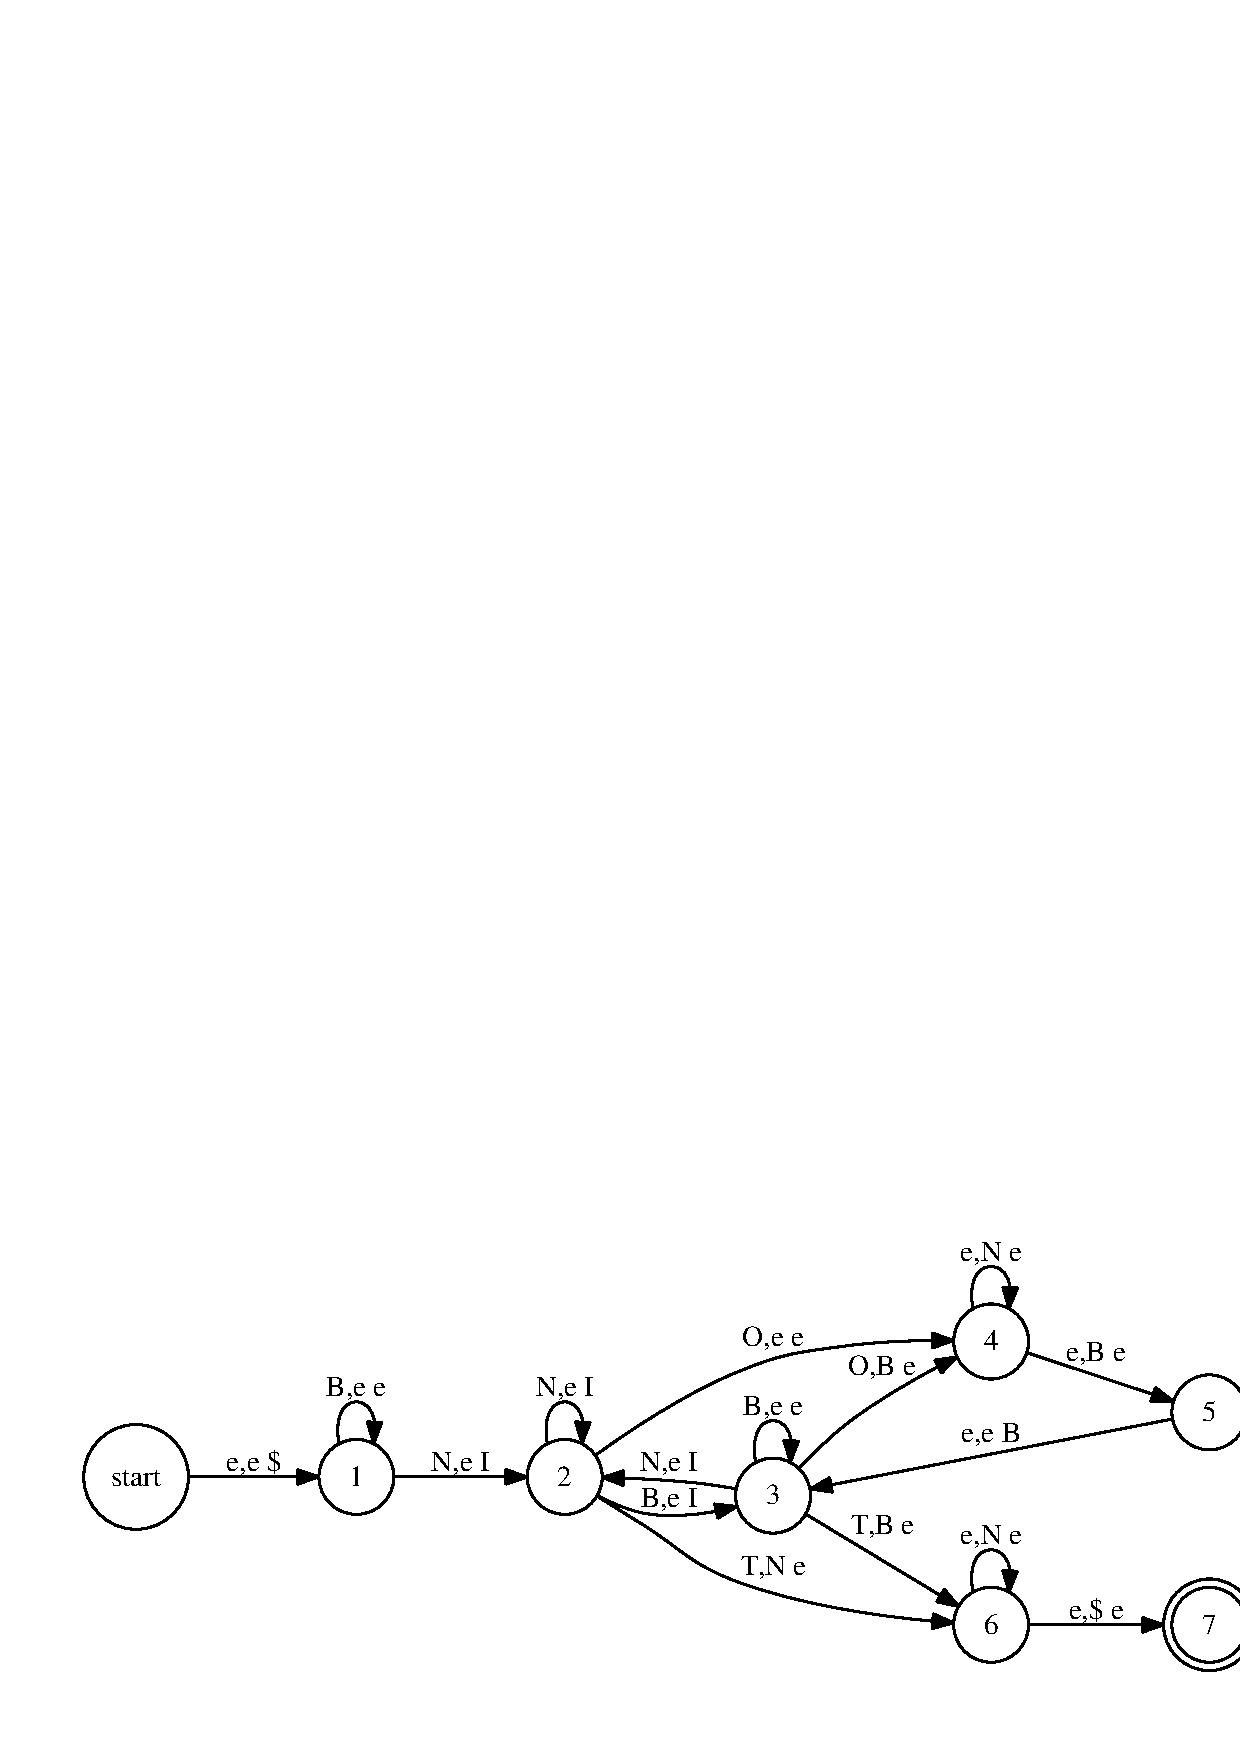
\includegraphics[width=\textwidth]{pda}
  \caption{Push Down Automata for Reverse Polish Notation.}
\end{figure}


Alternatively, \textit{states} could also be implemented according to
the example 2.14 in Sipser \cite[p. 114]{sipser2012}: The state is
represented by triple nested table or
an aggregated array where there is a multi column for each letter in
the input alphabet with subgroups as the individual column for each
letter of the stack alphabet. Implementing a representation for this
model could be done with a nested table, an array, where the logic for
accessing the different levels is integrated in the code or a tree
structure. Such a representation has the advantage that it is directly
visible whether a transition for a certain state is already defined or
not as it has a unique location in the data structure. When choosing a
representation with states as mere containers for transitions, a
control mechanism to prevent assignment of duplicate transitions is
needed. 

\subsubsection{States}

Finally, it was chosen to implement states as containers for
transitions. A state has an numeric \textit{id} and a directed list
with potential transitions to proceed along. The state itself is a
\textit{struct}.




The interface of the \textit{state} is in the current version very
sparse. It contains just the function \textit{state\_create} (returns a
new state) and \textit{state\_addTransition} (to add transitions to the
state). 


\subsubsection{Transition}
A transition needs to know whether it matches the current
state, it needs to define how to modify the current state and the id
of the new state. In the final implementation, the transition is a
struct with function pointers for the \textit{alphabet}
functions. Further, the transition contains an int of the destination
state, \textit{destInt} and a char \textit{description}. Note that in
the current implementation, the transition does not need to know it's
source state, hence, it could be reused as long as the destination state
matches. However, after implementing the datatypes, it was found that
reusing transitions causes problems with the memory free functions: It
happend that a transition was attempted to be removed multiple
times causing memory errors. Hence, in the current version, for
simplicity, instead of reusing, multiple identical transitions were created.  
  

\begin{table}[]
\centering
\caption{The table below shows the transitions used for the Reversed
  Polish Notation Push Down Automaton. The letter \textit{e} is used
  for \textit{epsilon}, \textit{B} as \textit{blank}, the letter
  \textit{I} for pushing \textit{input} to the stack. Further the
  letter \textit{O} and \textit{N} stand for \textit{operator} and
  \textit{number} respectively. \textit{T} stands for \textit{terminal} 
  and indicates the end of the input. The dollar sign is used as a
  letter of the stack alphabet to mark the first position. The column
  \textit{id} shows the id number of the transition in the C program.}
\label{tab:trans}
\begin{tabular}{llllll}
id  & source & destination & read & pop & push \\ \hline
1   & start  & 1           & e    & e   & \$    \\
2   & 1      & 1           & B    & e   & e    \\
3\_1 & 1      & 2           & N    & e   & I    \\
3\_2 & 2      & 2           & N    & e   & I    \\
5   & 2      & 3           & B    & e   & I    \\
4   & 2      & 4           & O    & e   & e    \\
6   & 2      & 6           & T    & N   & e    \\
3\_3 & 3      & 2           & N    & e   & I    \\
14  & 3      & 3           & B    & e   & e    \\
7   & 3      & 4           & O    & B   & e    \\
8   & 3      & 6           & T    & B   & e    \\
9   & 4      & 4           & e    & N   & e    \\
10  & 4      & 5           & e    & B   & e    \\
11  & 5      & 3           & e    & e   & B    \\
12  & 6      & 6           & e    & N   & e    \\
13  & 6      & 7           & e    & \$   & e   
\end{tabular}
\end{table}

The interface of the transition contains merely one function of
interest for the user, \textit{transition\_create}. All further
functions are used internal to check and apply the transitions. This
includes three functions to check for epsilon condition in the
transitiona (\textit{transition\_checkReadEpsilon,
  transition\_checkPopEpsilon, transition\_checkPushEpsilon}) and three
functions that wrap the \textit{alphabet} functions for input, stack
and push condition. 

\subsubsection{RPN Calculation Function}
As mentioned earlier, it was chosen to separate verification of the
input by the PDA from the calculation. The calculation is done by the
function \textit{rpn\_calc}. This function assumes that the input
statement is a valid RPN expression, hence the input is not
validated and it should as such just be used in conjunction with the
PDA datatype.

Compared to the PDA, the stack of the RPN calculator holds also multi
digit integers. In fact, integers are written to the stack just after
they are completely read and composed from the input. Blanks are
interpreted as number terminators. In beginning of the input, after
operators and after terminating a number read, blanks are
disregarded. This behaviour agrees with the implemented rule set in
the PDA. 

The parsing of \textit{char} type operators into real aritmethic
operators was inspired by a \textit{Stack Overflow} blog post \cite{lookup}.

\section{Testing}
A range of different inputs where tested. The testcases can be found
in \textit{table \ref{tab:test}}.

\begin{table}[]
\centering
\caption{Test cases}
\label{tab:test}
\begin{tabular}{lll}
expression          & expected           & test \\ \hline
``''                  & Invalid expression & ok   \\
``1''                 & 10                 & ok   \\
``0''                 & 0                  & ok   \\
``01''                & 1                  & ok   \\
``1 1''               & Invalid expression & ok   \\
``a1''                & Invalid expression & ok   \\
``0 1/''              & 0                  & ok   \\
``   1 1  +  ''       & 2                  & ok   \\
``11111 11111*''      & 1234554321         & ok   \\
``111111 111111*''    & -539247567         & ok   \\
``10 20-''            & -10                & ok   \\
``1 2 + 3 - 4 * 5 /'' & 0                  & ok   \\
``1 2 3 +''           & Invalid expression & ok   \\
``*''                 & Invalid expression & ok  
\end{tabular}
\end{table}

\section{Extra Assignment - Bracket Matching}
After the basic datatypes and the RPN automaton were implemented, it
was tested how flexible the program would be for another
automaton. For this reason the \textit{Bracket Matching} automaton was
implemented. After copying the \textit{main} program of the RPN
automaton, adjusting took just a few minutes. Basically, three states
and five transitions had to be set.  Addiontally, three new
\textit{alphabet} functions had to be written:
\textit{isOpeningBracket}, \textit{isClosingBracket} and
\textit{openingBracket}. Finally, the RPN calculation function was removed from
main. The program uses all the same header files and is available in
the file \textit{bracket\_automat.c}. For testing, the expressions
given in the labdescription were used. 

\section{Discussion}
The chosen design is very flexible for implementing generic automata
as demonstrated with the \textit{Bracket Matching} automaton. The
chosen separation of datatypes works well and allows for quick
reconfiguration of the automaton. It can be argued whether the
\textit{State} datatype is needed at all. Instead one could include
also the source state in the transitions. Also the information about
accepted / non-accepted state could be included in the
transitions. This would however result in more redundant information
and the need for validating it to prevent wrong user input.

Admittedly, as mentioned in the description to the lab assignment, 
a grpah would probably have been a more natural basis for this
datatype. 


\addcontentsline{toc}{section}{\refname}
\bibliography{references}

\end{document}
